\chapter{Introdução}\label{CAP:introducao}

\noindent O desenvolvimento de uma redação e uma atividade prática presente na cultura civilizada desde a invenção da escrita.
Já faz pelo menos uma década que um bom desempenho na redação do Exame Nacional de Ensino Médio - ENEM  virou sinônimo de chances maiores para ser aprovado no processo seletivo de acesso a inúmeras universidades públicas ~\cite{sisu:2017} e a importantes programas de governo como Ciência sem fronteiras ~\cite{csf:2017}.

Em todo processo seletivo é comum o uso de marcações em gabaritos afim de automatizar o processo de correção, uma alternativa rápida e segura, até mesmo aplicações de provas eletrônicas são cada vez mais comum. Um exemplo seria o processo seletivo para avaliador das redações do ENEM que durante a ``FASE II'' respondem uma prova eletrônica eliminatória ~\cite{paq_a:2016}. É notável que todo o processo evoluiu com objetivo de agilidade, confiança e segurança do resultado, entretanto a avaliação das competências de uma redação ainda depende exclusivamente da supervisão de duas ou mais pessoas envolvidas ~\cite{edital_enem:2016}.

A redação é aplicada no ENEM desde a primeira edição 1998, hoje o maior exame do Brasil, que na edição de 2016 teve 8.627.195 escritos confirmados, e a participação direta de 11.360 profissionais externos na correção de 5.825.134 redações, entre eles, 378 supervisores e 10.982 avaliadores de acordo com a CEBRASPE ~\cite{relatorio_de_gestao:2016}. 

Segundo o edital do ENEM 2016 ~\cite{edital_enem:2016} cada redação foi avaliada por, pelo menos, dois avaliadores, de forma independente, contabilizando um número mínimo de 11.650.268 avaliações manuais, das competências exigidas em um texto de redação pelo ENEM.

\textit{Machine Learning} ou aprendizado de máquina é uma área de IA cujo objetivo é o desenvolvimento de técnicas computacionais sobre o aprendizado bem como a construção de sistemas capazes de adquirir conhecimento de forma automática. Os algoritmos de aprendizado de máquina procuram padrões dentro de um conjunto de dados~\cite{machine_learning:1997}. Esses algoritmos existem há bastante tempo, uma ciência que não é nova, mas que está ganhando um novo impulso enquanto o processamento computacional cresce e fica mais barato.

A hipótese desta monografia é que um ou mais modelos de aprendizado de máquina na valoração das competências de uma redação pode ser tão eficiênte quanto o processo de avaliação manual.

\section{Definição do Problema de Pesquisa}

Dado um corpus de redações avaliar as competências exigidas em um texto de redação do tipo dissertativo-argumentativo substituindo a etapa de avaliação manual.

\section{Motivação}

Com crescente volume e variedade de dados disponíveis, o processamento computacional que está mais barato e mais poderoso, e o armazenamento de dados de forma acessível, o aprendizado de máquina está no centro de muitos avanços tecnológicos atingindo áreas antes exclusivas de seres humanos. Os carros autônomos do Google são o exemplo de uma atividade antes exclusiva de um humano e hoje exercida e aperfeiçoada por algoritmos de aprendizado de máquina ~\cite{waymo:2017}.

Aplicações de aprendizado de máquina estão presentes na nossa vida cotidiana como, resultados de pesquisa web, análise de sentimento baseado em texto e na detecção de fraudes em operações com cartões de crédito ~\cite{batista1999aplicando}.

As competências exigidas em uma redação podem ser avaliadas por aprendizado de máquina. Diferente de um ser humano um algoritmo de aprendizado de máquina está livre de ansiedade, fadiga, \textit{stress} entre outro fatores emocionais que afetão uma avaliação. Isto representaria a classificação de um texto imparcial a opinião do autor classificando todas as competências necessárias para definição de uma nota.

\section{Objetivos Gerais e Específicos}

Este trabalho tem como objetivo geral aplicar aprendizado de máquina na avaliação das competências exigidas em um texto de redação do tipo dissertativo-argumentativo.

\subsection{Objetivos Especificos}

Dentro do escopo geral de forma detalhada e refinada as ações que se prentende executar para alcançar o objetivo geral acima, são particularizadas como os seguintes objetivos específicos:

\begin{itemize}
 \item Percorrer o banco de redações UOL ~\cite{uol_banco_redacoes:2017}, filtrar e coletar redações avaliadas;
 \item Normalizar os textos coletados separar o tema, título, texto e competências avaliadas em uma estrura no formato JSON e armazenar;
 \item Montar um fluxo de trabalho utilizando a ferramenta de \textit{Data Mining} Orange3 com modelos  classificadores de multiplas classes;
 \item Ajustar e treinar os modelos classificadores com o corpus de redações; 
 \item Realizar testes de acurácia, \textit{overfitting} e \textit{noise};
  \begin{itemize}
   \item Acurácia ou taxa de erro;
   \item \textit{Overfitting} ou super-ajustamento;
   \item \textit{Noise} ou ruído;
  \end{itemize}
 \item Representar graficamente os resultados obtidos. 
\end{itemize}

\section{Metodologia}

Para concluir com êxito os objetivos propostos o método utilizado para solução do problema tem os seguintes passo:

\begin{figure}[h]
\begin{center}
    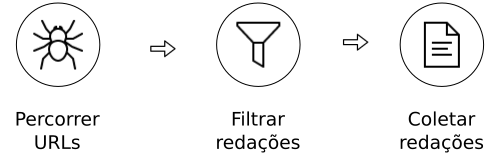
\includegraphics[scale=0.75]{figuras/metodologia_1.png}
\end{center}
\caption{Diagrama de blocos da primeira etapa.}
\label{Img:3DRobotWorkspace}
\end{figure}

\begin{figure}[h]
\begin{center}
    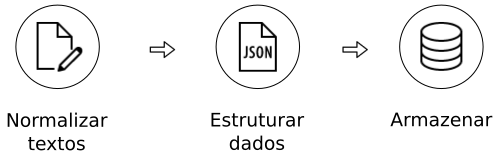
\includegraphics[scale=0.75]{figuras/metodologia_2.png}
\end{center}
\caption{Diagrama de blocos da segunda etapa.}
\label{Img:3DRobotWorkspace}
\end{figure}

\begin{figure}[h]
\begin{center}
    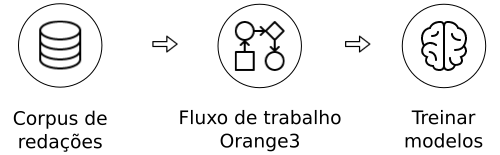
\includegraphics[scale=0.75]{figuras/metodologia_3.png}
\end{center}
\caption{Diagrama de blocos da terceira etapa.}
\label{Img:3DRobotWorkspace}
\end{figure}

\begin{figure}[h]
\begin{center}
    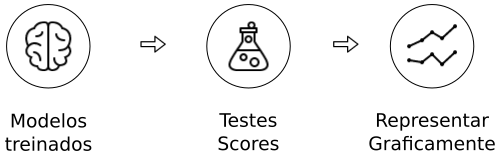
\includegraphics[scale=0.75]{figuras/metodologia_4.png}
\end{center}
\caption{Diagrama de blocos da quarta etapa.}
\label{Img:3DRobotWorkspace}
\end{figure}


% Normalizar os textos coletados tal que o valor textual ainda seja o mesmo que o original, mas cuja representação binária está no formato de normalização Unicode especificado,

% Será necessário realizar estudo e análise sobre o tema para obter o conhecimeto
% necessário para o desenvolvimento e conclusão de todos os objetivos propostos.

\section{Contribuicoes}




\section{Organizacao do trabalho}

\noindent \textbf{Capitulo \ref{trab_rela}}: descricao...

\noindent \textbf{Capitulo \ref{meto}}: descricaoo...

\noindent \textbf{Capitulo \ref{desen}}: descricao...

\noindent \textbf{Capitulo \ref{result}}: descricao...